\clearpage
\section{Architettura applicazione Android}

Per avere un overview generale dell'applicazione è utile osservare il seguente diagramma dei package: 

\begin{figure}[H]
	\begin{center}
		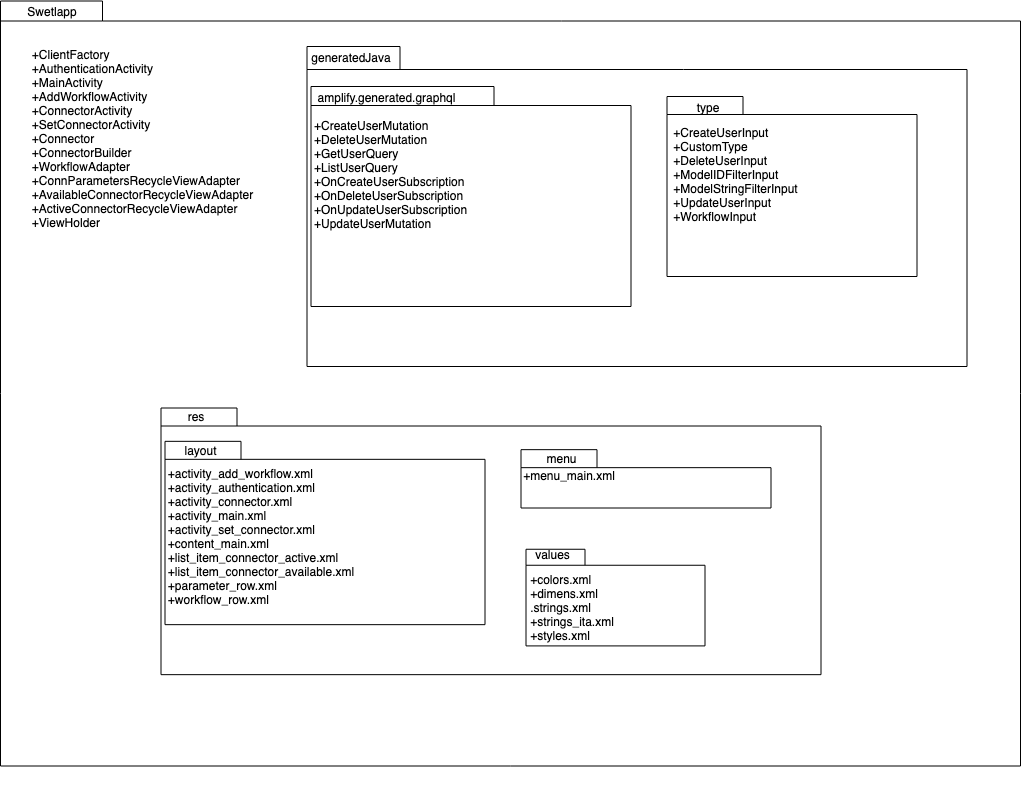
\includegraphics[width=0.75\textwidth, keepaspectratio]{../includes/pics/package_diagram.png}
		\caption{Package diagram SwetlApp}
	\end{center}
\end{figure}

L'applicazione contiene le seguenti activity:

\begin{itemize}
    \item \emph{AuthenticationActivity}: è la prima activity che viene aperta dall'app, permette la registrazione, il login e verifica se l'utente è loggato o meno. Il form di inserimento dei dati e la loro gestione è generato da AWS Cognito;
        \begin{figure}[H]
        \begin{center}
            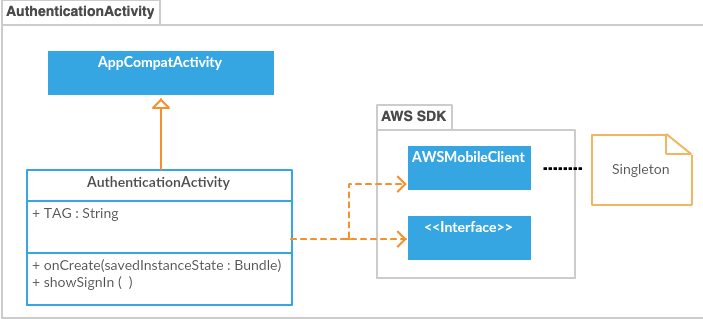
\includegraphics[width=0.9\textwidth, keepaspectratio]{../includes/pics/authenticationactivity.png}
            \caption{Diagramma della classe AutenticationActivity}
        \end{center}
        \end{figure}


   \item \emph{MainActivity}: è la schemata principale che mostra la lista di Workflow dell'utente;
        \begin{figure}[H]
	    \begin{center}
		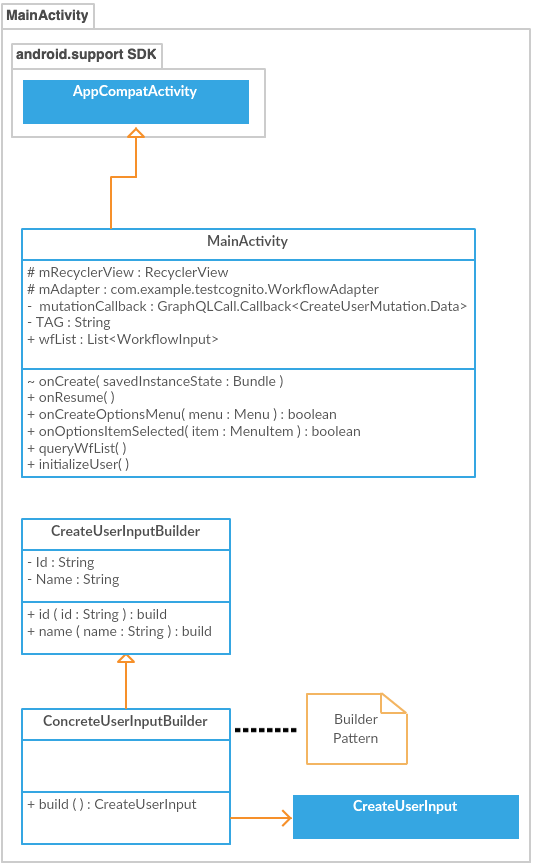
\includegraphics[width=0.8\textwidth, keepaspectratio]{../includes/pics/mainactivity.png}
		\caption{Diagramma della classe MainActivity}
	    \end{center}
        \end{figure}
        

    \item \emph{AddWorkflowActivity}: è l'activity che consente di inserire un nuovo workflow;
       \begin{figure}[H]
	   \begin{center}
    
		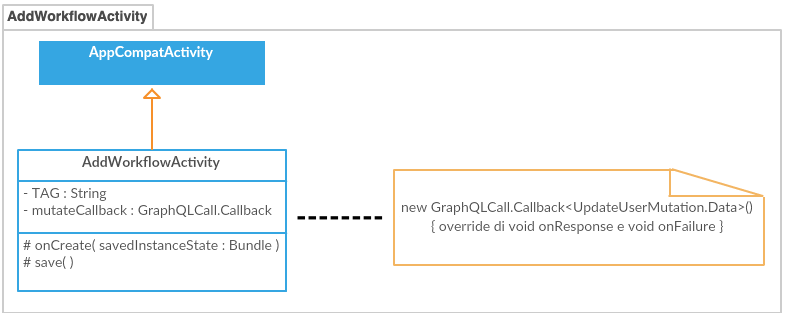
\includegraphics[width=0.9\textwidth, keepaspectratio]{../includes/pics/addworkflowactivity.png}
		\caption{Diagramma della classe AddWorkflowActivity}
	   \end{center}
       \end{figure}
   
   
   
    \item \emph{ConnectorActivity}: è l'activity che consente di gestire i connettori relativi al workflow su cui si sta operando;
        \begin{figure}[H]
	    \begin{center}
		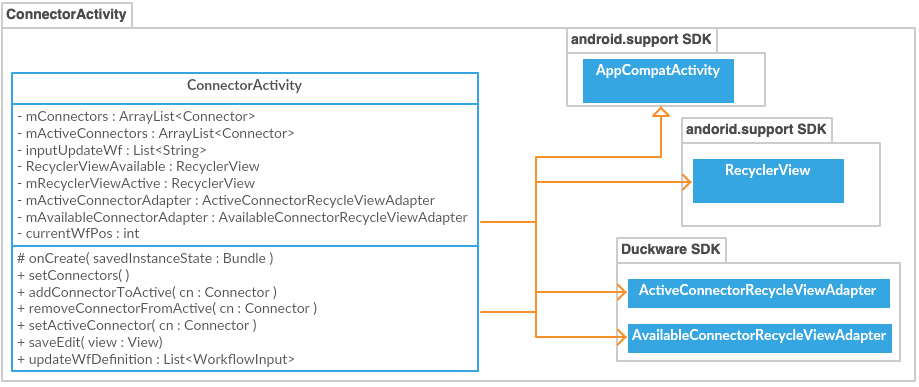
\includegraphics[width=0.9\textwidth, keepaspectratio]{../includes/pics/connectoractivity.png}
		\caption{Diagramma della classe ConnectorActivity}
	    \end{center}
        \end{figure}
    
    
     \item \emph{SetConnectorActivity}: è l'activity che consente di gestire i parametri relativi al connettore su cui si sta operando;
        \begin{figure}[H]
	    \begin{center}
		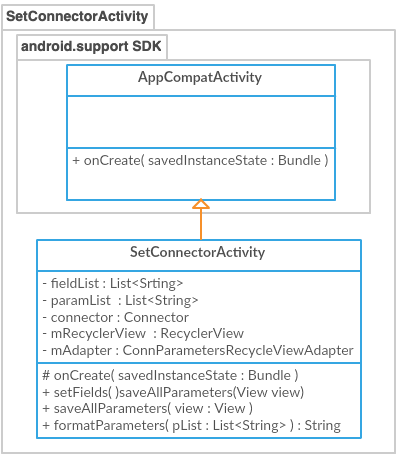
\includegraphics[width=0.9\textwidth, keepaspectratio]{../includes/pics/setconnectoractivity.png}
		\caption{Diagramma della classe SetConnectorActivity}
	    \end{center}
        \end{figure}   
\end{itemize}

È inoltre presente la classe di supporto Connector.java non generata automaticamente da Amplify:
        \begin{figure}[H]
	    \begin{center}
		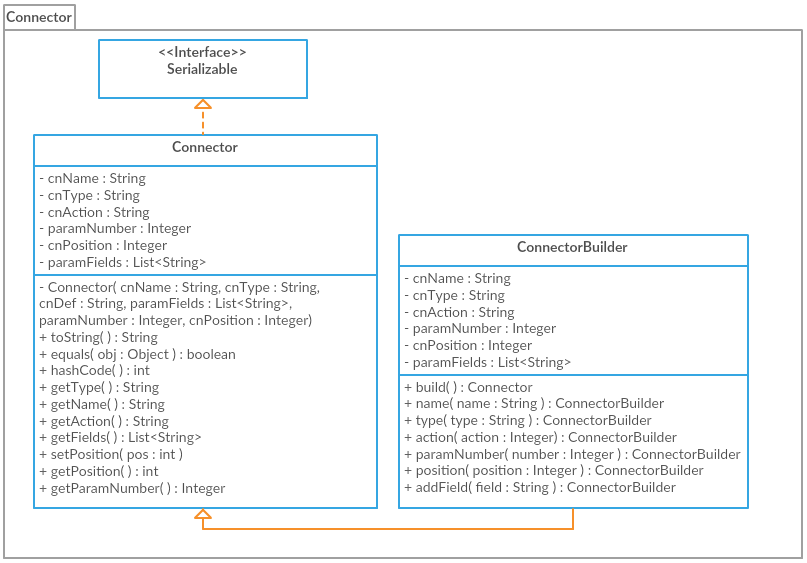
\includegraphics[width=0.75\textwidth, keepaspectratio]{../includes/pics/connector.png}
		\caption{Diagramma della classe Connector}
	    \end{center}
        \end{figure}
        
Questa utilizza un builder pattern poichè i connettori vengono istanziati con attributi eterogenei e a volte vuoti.        

Ogni Activity potrà comunicare con le API solamente utilizzando il client generato dalla classe \emph{ClientFactory}.\\[0.25cm]

\begin{figure}[H]
	\begin{center}
		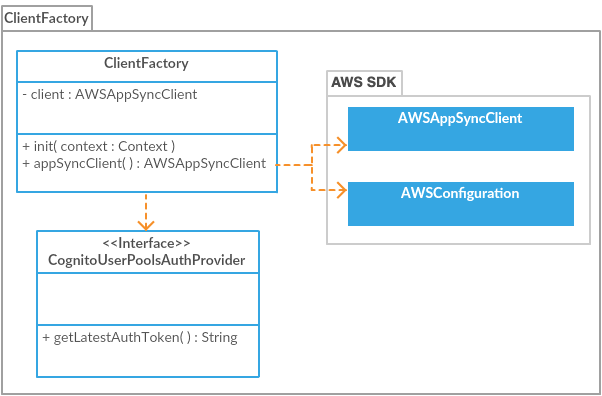
\includegraphics[width=0.9\textwidth, keepaspectratio]{../includes/pics/clientfactory.png}
		\caption{Classe ClientFactory}
	\end{center}
\end{figure}

Le risorse dellínterfaccia grafica sono definite nel namespace res e comprendono i file in linguaggio xml che descrivono gli elementi delle view (layout) e i valori importati da questi elementi (values) quali: 
\begin{itemize}
\item colori;
\item dimensioni;
\item stili;
\item stringhe per lingua italiana;
\item stringhe per lingua inglese;
\end{itemize}



Oltre alle activity e alle risorse xml , è importante notare che tutto il codice necessario alle operazioni sulle risorse backend è definito nel namespace generatedJava, tutto il codice contenuto in questo namespace è generato in automatico da Amplify.

\subsection{Amplify}

Amplify è il framework di Amazon utilizzato per generare un SDK che permette la comunicazione dell'applicazione Android con i servizi in cloud di AWS. La CLI di Amplify consente di sincronizzare i servizi online con l'applicazione, generare librerie di supporto e fornire strumenti di test allo sviluppatore.

\begin{figure}[H]
	\begin{center}
		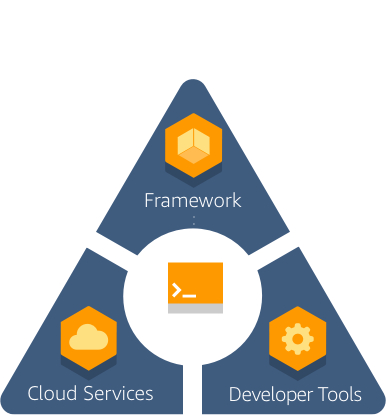
\includegraphics[width=0.55\textwidth, keepaspectratio]{../includes/pics/amplify.png}
		\caption{AWS Amplify}
	\end{center}
\end{figure}

L'integrazione di Amplify in Android Studio consente di delegare controllo e creazione del backend dell'applicazione, noi abbiamo utilizzato Amplify principalmente per due funzioni:

\begin{itemize}
    \item aggiunta di AWS Cognito.
    \item aggiunta di API GraphQL.
\end{itemize}

I metodi per interfacciarsi con Cognito vengono forniti da una libreria di Amazon mentre i metodi per fare query e mutazioni all'endpoint GraphQL vengono generati da Amplify.


Questo è un esempio di query per inserire dati relativi ad un utente:

\begin{verbatim}
     CreateUserInput input = CreateUserInput.builder()
                  .id(AWSMobileClient.getInstance().getUsername())
                  .name(AWSMobileClient.getInstance().getTokens()
                  		.getIdToken().getClaim("nickname"))
                  .build();

        CreateUserMutation addUserMutation = CreateUserMutation.builder()
                .input(input)
                .build();
        com.example.swetlapp.ClientFactory.appSyncClient()
        			.mutate(addUserMutation).enqueue(callback);
\end{verbatim}

CreateUserInput e CreateUserMutation sono due classi generate da Amplify, entrambe sono costruibili tramite builder pattern, AWSMobileClient (singleton) ci permette di comunicare con la user pool di AWS Cognito e ci ritorna informazioni relative all'utente. Quindi si crea l'input per la mutazione, si crea la mutazione stessa, infine esegue questa utilizzando come oggetto di invocazione l'istanza di ClientFactory ritornata dal metodo appSyncClient().\\
Lo schema generale per "comunicare" con le risorse è sempre questo (a meno di query di sola lettura in cui non è necessario costruire un input).


\subsection{Generazione API}

Le API nel nostro caso corrispondono a una soluzione per richieste HTTP ad un endpoint GraphQL.
Per creare e accedere alle API è necessario il servizio AWS AppSync, anche questo sarà settato da amplify.
Componenti principali di AppSync sono:
\begin{itemize}
\item un proxy GraphQl che processa le richieste e le mappa su funzioni e trigger;
\item operazioni: query e mutazioni;
\item data source: nel nostro caso DynamoDB;
\item resolver: converte operazioni GraphQL per essere eseguite sul data source effettivo;
\item AppSync client: dove sono definite le operazioni GraphQL;
\end{itemize}

L'ordine degli eventi per l'impostazione del backend è questo:

\begin{itemize}
\item settaggio di un endpoint GraphQL tramite CLI Amplify;
\item scrittura dello schema delle risorse in linguaggio GraphQL Schema;
\item pubblicazione dello schema;
\item generazione delle API su AppSync (automatico)
\item generazione del database DynamoDB (automatico)
\item generazione dell'SDK per effettuare operazioni definite dallo schema GraphQL (automatico)
\end{itemize}

Lo schema GraphQL che abbiamo scritto è il seguente:
\begin{verbatim}
type User @model {
  id: ID!
  name: String!
  workflow: [Workflow!]
}

type Workflow {
  idwf: ID!
  name: String
  def: String
}
\end{verbatim}


A partire da questo, in dynamoDB è stata generata una tabella User con i campi:
\begin{itemize}
\item id;
\item name;
\item lista di workflow;
\end{itemize}

Amplify genera solo le classi java dei tipi con direttiva \textit{@model}, quindi abbiamo a disposizione solo operazioni con il tipo User, per accedere ai workflow, ai connettori dei workflow e ai parametri dei connettori è necessario operare con il file Json definito dalla stringa \textit{def}, per operare agevolmente con i file Json in ambiente Android abbiamo importato le librerie \textit{import org.json.JSONException} e \textit{import org.json.JSONObject}.

Esempio: per generare il Json nella forma:

\begin{verbatim}
{\"action\":\"connector_action\",\"params\":[\"first_param\",\"second_param\"]}
\end{verbatim}

il codice Java sarà:

\begin{verbatim}
            Map<String, Object> connMap = new HashMap<>();
            connMap.put("action",connector.getAction());
            connMap.put("params",pList);
            JSONObject jsonObject = new JSONObject(connMap);
\end{verbatim}



